\documentclass[varwidth=true, border=2pt]{standalone}
\usepackage{tikz}

\begin{document}
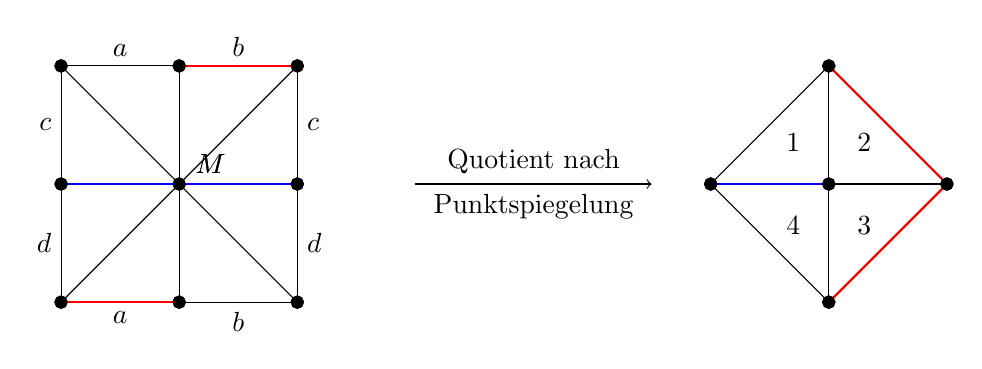
\begin{tikzpicture}[scale=1.5]
    \tikzstyle{point}=[circle,thick,draw=black,fill=black,inner sep=0pt,minimum width=4pt,minimum height=4pt]
    \node (a)[point] at (0,0) {};
    \node (b)[point] at (1,0) {};
    \node (c)[point] at (2,0) {};

    \node (d)[point] at (0,1) {};
    \node (M)[point,label={[label distance=0cm]5:$M$}] at (1,1) {};
    \node (f)[point] at (2,1) {};

    \node (g)[point] at (0,2) {};
    \node (h)[point] at (1,2) {};
    \node (i)[point] at (2,2) {};

    \draw (a.center) -- node[below] {$a$} (b.center);
    \draw (b.center) -- node[below] {$b$} (c.center);
    \draw (g.center) -- node[above] {$a$} (h.center);
    \draw (h.center) -- node[above] {$b$} (i.center);
    \draw (d.center) -- node[left] {$c$} (g.center);
    \draw (d.center) -- node[left] {$d$} (a.center);
    \draw (f.center) -- node[right] {$d$} (c.center);
    \draw (i.center) -- node[right] {$c$} (f.center);

    \draw (a.center) -- (b.center) -- (M.center) -- (d.center) -- cycle;
    \draw (b.center) -- (c.center) -- (f.center) -- (M.center) -- cycle;
    \draw (d.center) -- (M.center) -- (h.center) -- (g.center) -- cycle;
    \draw (M.center) -- (f.center) -- (i.center) -- (h.center) -- cycle;

    \draw[thick, blue] (d.center) -- (M.center) -- (f.center);

    \draw[thick, red] (a.center) -- (b.center);
    \draw[thick, red] (h.center) -- (i.center);

    % Draw again so that lines are below nodes
    \draw (a.center) -- (i.center);
    \draw (c.center) -- (g.center);

    \node (a)[point] at (0,0) {};
    \node (b)[point] at (1,0) {};
    \node (c)[point] at (2,0) {};

    \node (d)[point] at (0,1) {};
    \node (M)[point,label={[label distance=0cm]5:$M$}] at (1,1) {};
    \node (f)[point] at (2,1) {};

    \node (g)[point] at (0,2) {};
    \node (h)[point] at (1,2) {};
    \node (i)[point] at (2,2) {};

    \draw[->] (3,1) -- node[above] {Quotient nach} node[below] {Punktspiegelung} (5,1);

    \begin{scope}[xshift=6.5cm,yshift=1cm]
        \node (w)[point] at (-1,0) {};
        \node (x)[point] at (0,-1) {};
        \node (y)[point] at (1,0) {};
        \node (z)[point] at (0,1) {};
        \node (m)[point] at (0,0) {};

        \node (1) at (-0.3,+0.35) {1};
        \node (2) at (+0.3,+0.35) {2};
        \node (3) at (+0.3,-0.35) {3};
        \node (4) at (-0.3,-0.35) {4};

        \draw (w.center) -- (x.center) -- (y.center) -- (z.center) -- cycle;

        \draw[thick, blue] (w.center) -- (m.center);
        \draw (m.center) -- (y.center);
        \draw (x.center) -- (m.center) -- (z.center);
        \draw[thick, red] (z.center) -- (y.center) -- (x.center);

        % Draw again, as lines should be below points
        \node (w)[point] at (-1,0) {};
        \node (x)[point] at (0,-1) {};
        \node (y)[point] at (1,0) {};
        \node (z)[point] at (0,1) {};
        \node (m)[point] at (0,0) {};
    \end{scope}
\end{tikzpicture}
\end{document}
